A toy model of AOD provides a simple-to-understand representation for how real and Monte Carlo simulated data will react under optimization conditions for derivation production jobs. 
One commonality between both data and MC is the branch data within both is made of a mixture between repeated integer-like data and randomized floating-point data (i.e. data that has both easily and difficult to compress.)
Replicating this mixture of data in a branch would give us an effective model that would resemble how current derivation jobs would act on real and MC simulated data. 
These toy model mixtures would provide an avenue to test opportunities for optimizing the demand on the GRID by first looking at limiting basket sizes and their effects on compression of branches. 

\section{Introducing the Toy Model}

There were a number of iterations to the toy model, but the first was constructed by filling up a TTree with branches that each have vectors with varying number of random floats written and read back.
This original model had four distinct branches, each with a set number of events ($N=1000$), and each event having a number of entries, vectors with 1, 10, 100, and 1000 floats each.
Specifics are illustrated in Appendix \ref{appendix:toy_model_no_mix_code}.

% How we compressed these was through calling AutoFlush
Once the branches were filled, ROOT then will loop over each of the branches in the TTree and at regular intervals will remove the baskets from memory, compress, and write the baskets to disk (flushed), as was discussed in Section $\S \ref{section: ATLASIO_TTreeObject}$.
%  the compression factor for each branch that was filled.
To reiterate, the goal was to create branches with data similar to what could be found in real post-reconstructed data samples.
This would mean creating for branches with compression ratios on the order $\mathcal{O}(5)$, as is typical for such real data. 


\section{Toy Model Compression}

\subsection{Random Float Branches}

Upon reading back the ROOT file, the user would be able to see the original size of the file (Total-file-size), the compressed file size (File-size), the ratio between Total-file-size and File-size (Compression Factor), the number of baskets per branch, the basket size, and other information. 
Since the branches had vectors with exclusively random floats, it becomes apparent that the more randomization in the branches the harder it is to compress. 

\begin{figure}[h]
    \centering
    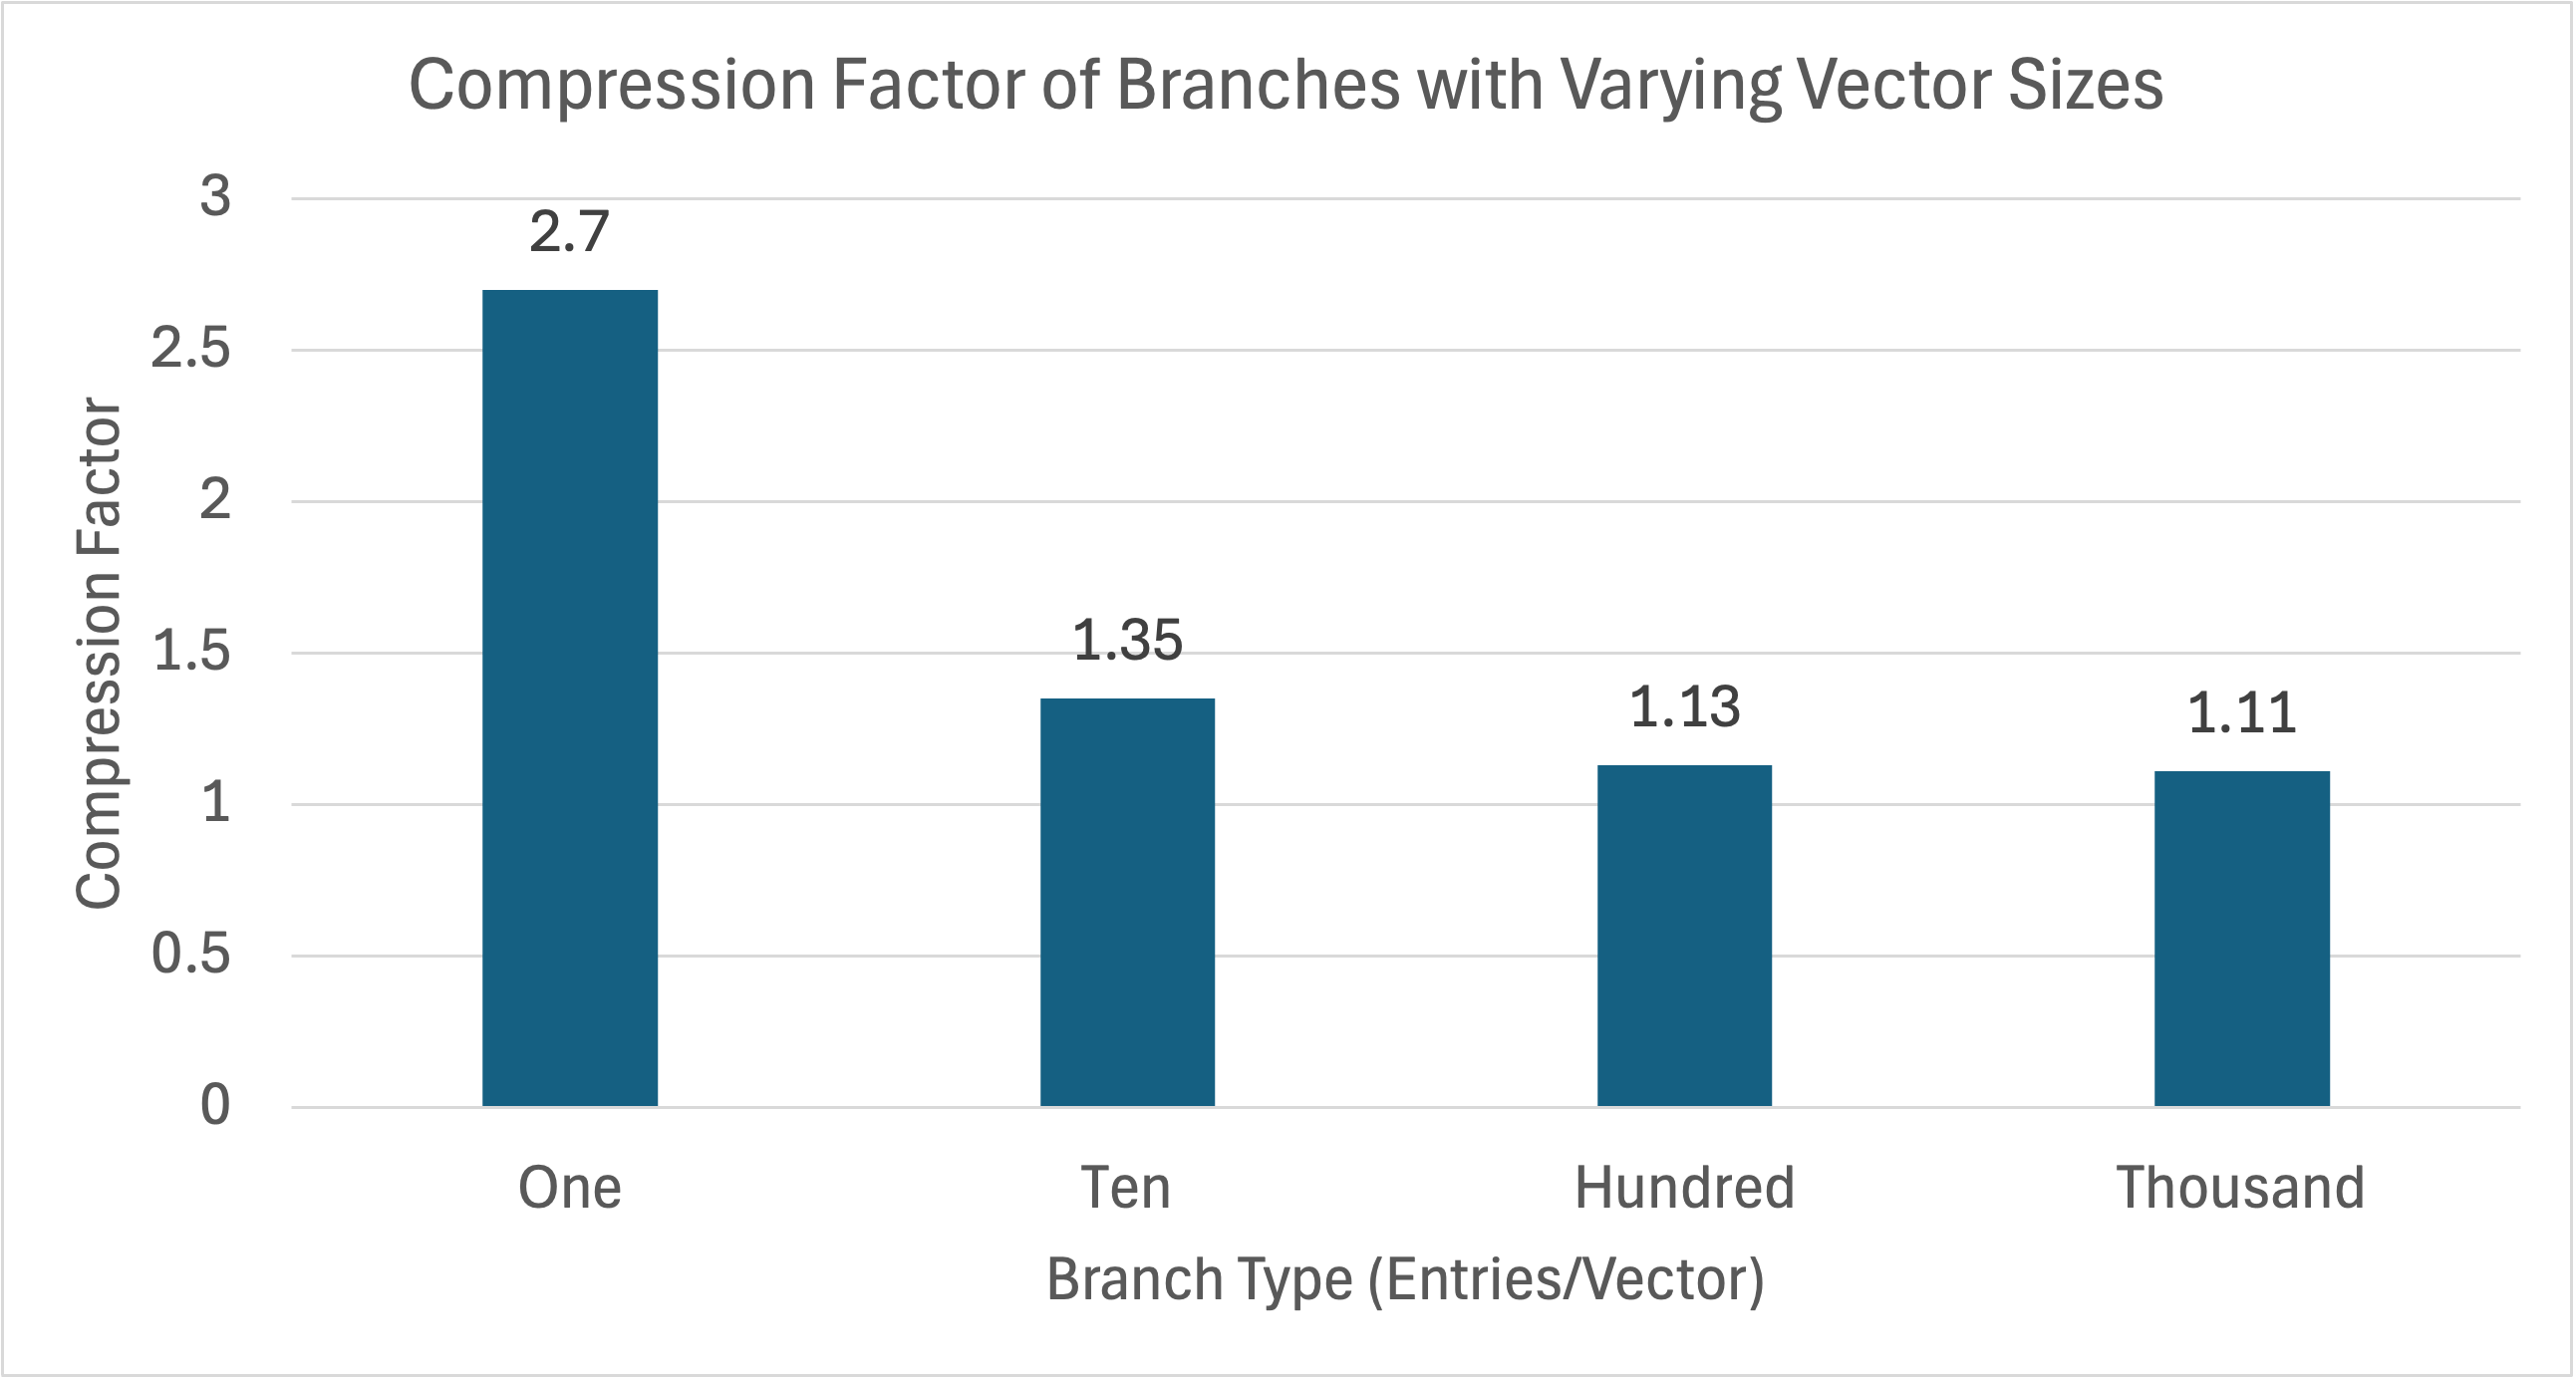
\includegraphics[width=.8\textwidth]{content/toymodel_content/branch_compfacts_nomix.png}
    \caption{Compression factors of $N=1000$ entries per branch with random-valued vectors of varying size.}
    \label{fig:toymodel_compF_rndm_vectors}
\end{figure}

% \begin{figure}[h]
%     \caption{File size of $N=1000$ entries per branch with random-valued vectors of varying size.}
%     \label{fig:toymodel_filesize_rndm_vectors}
%     \centering
%     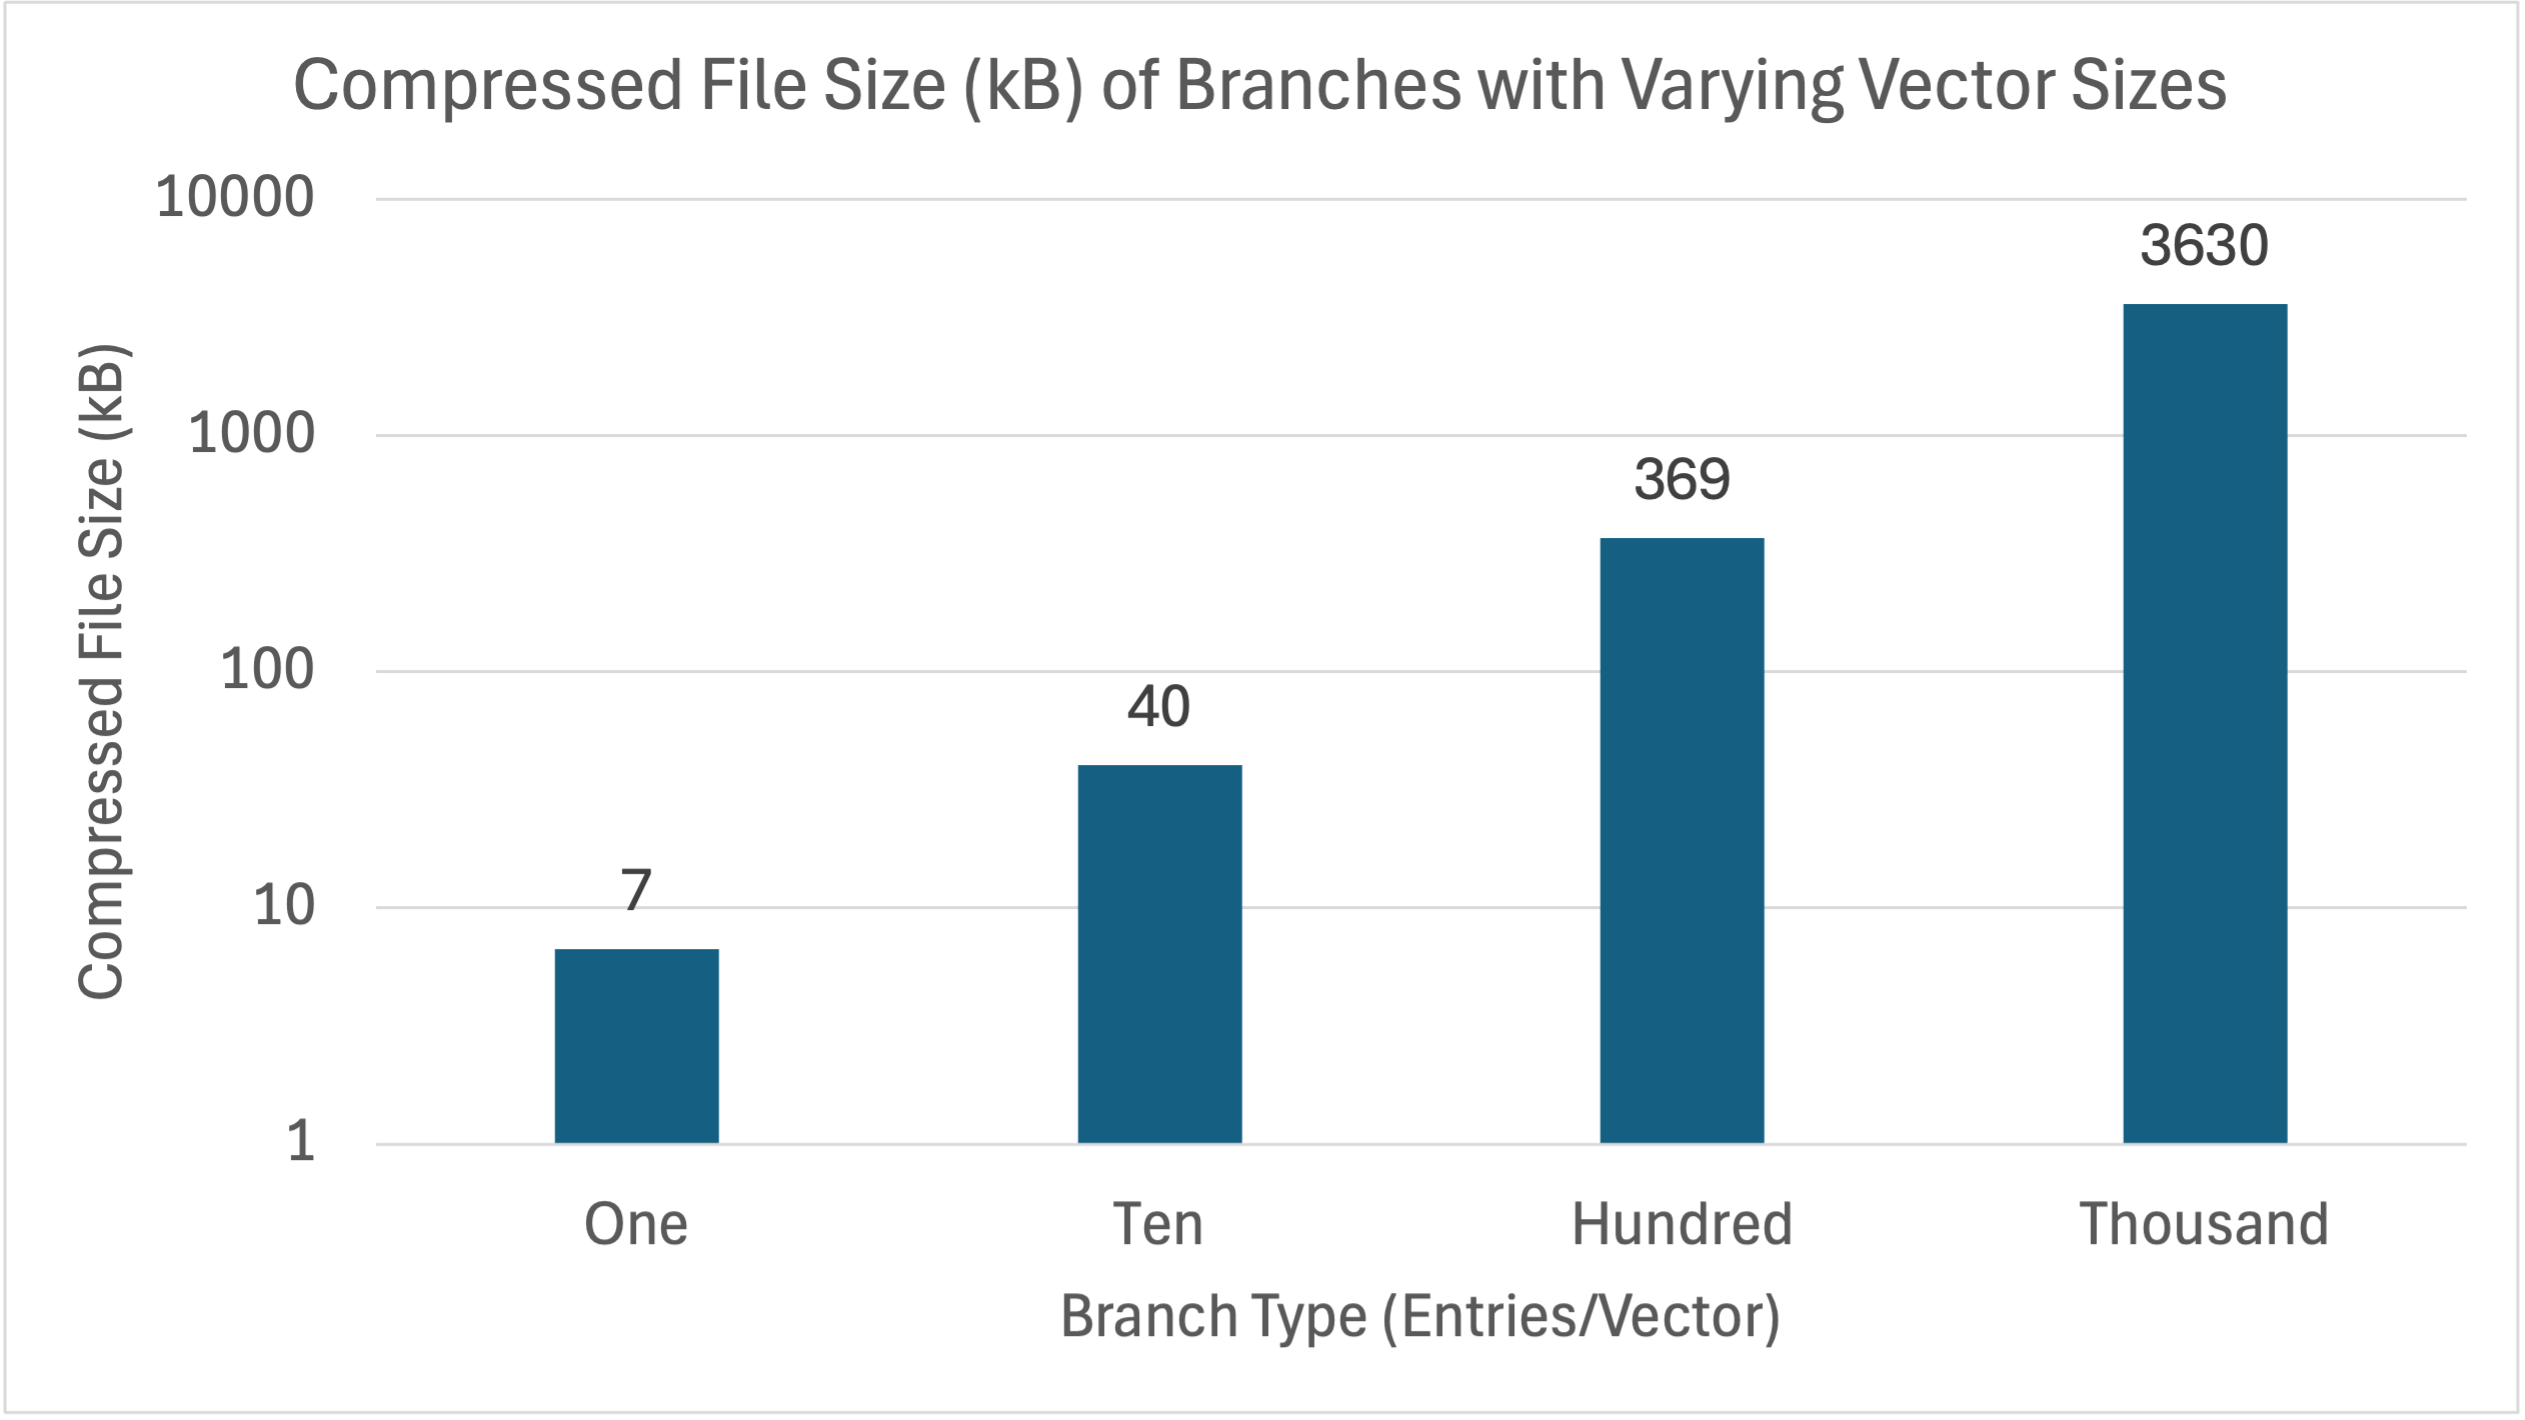
\includegraphics[width=.8\textwidth]{content/toymodel_content/branch_fileSize_nomix.png}
% \end{figure}

Figure \ref{fig:toymodel_compF_rndm_vectors} shows compression drop-off as the branches with more randomized floats per vector were present.
This is the leading indication that there needs to be more compressible data within the branches. 

\subsection{Mixed-Random Float Branches}
The branches needed to have some balance between compressible and incompressible data to mimic the compression ratio found in real data.
How this was achieved was by filling each vector with different ratios of random floats and repeating integers, see code in Appendix \ref{appendix:toy_model_WITH_mix_code}.
The first attempt creating branches with mixed amounts of randomization was having a mixture of 1/2 random data at $N=10^6$ events. 
However that led to the larger branches still seeing poor compression, so a new mixture of 1/4 random data was introduced. 

Figure \ref{fig:toymodel_compF_1e6_mix_random} shows the difference between compression between the two mixtures. 
When the number of events is increased from $N=10^5$ to $N=10^6$, branches with only half of the mixture is random data become larger and the branches with more vectors per entry become more difficult to compress. 
Figure \ref{fig:toymodel_compF_1e5_mix_random} shows a compression ratio hovering around 3 for the larger branches, whereas Figure \ref{fig:toymodel_compF_1e6_mix_random} shows the same branches hovering around 2. 

\begin{figure}[h]
    \centering
    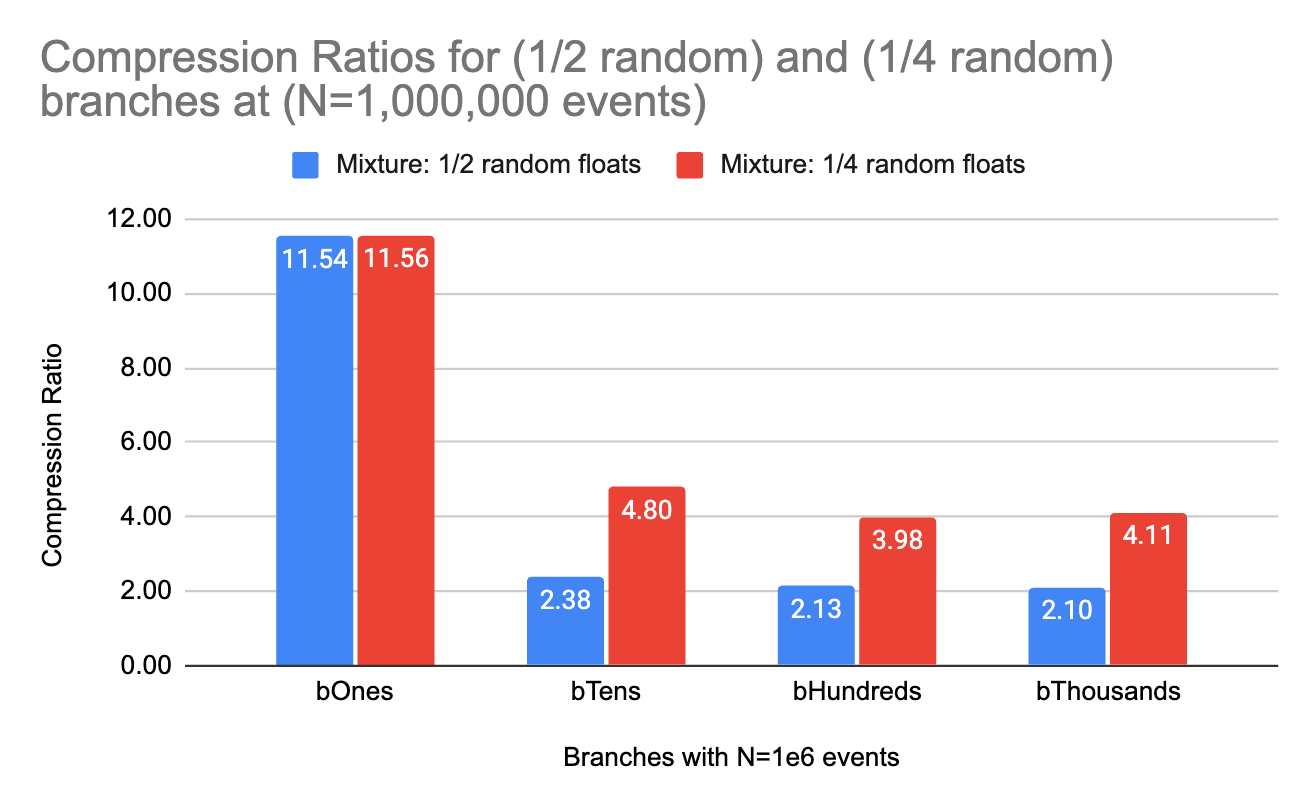
\includegraphics[width=.8\textwidth]{content/toymodel_content/Compression Ratios for (1_2 random) and (1_4 random) branches at (N=1,000,000 events).png}
    \caption{Compression Ratios for ($\frac{1}{2}$ random) and ($\frac{1}{4}$ random) branches at ($N=10^6$ events)}
    \label{fig:toymodel_compF_1e6_mix_random}
\end{figure}

\begin{figure}[h]
    \centering
    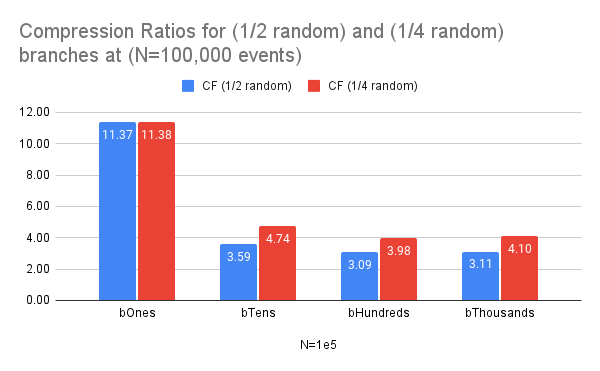
\includegraphics[width=.8\textwidth]{content/toymodel_content/Compression Ratios for (1_2 random) and (1_4 random) branches at (N=100,000 events).png}
    \caption{Compression Ratios for ($\frac{1}{2}$ random) and ($\frac{1}{4}$ random) branches at ($N=10^5$ events)}
    \label{fig:toymodel_compF_1e5_mix_random}
\end{figure}

Unlike the mixture of branches having 1/2 random data, the 1/4 mixture does not see the same compression effect, but with this mixture we see a compression ratio that is in-line with real data.
It was still worth testing the $N=10^6$ events for stress testing purposes.
Here is where tuning the basket size can begin to start.

\section{Basket-Size Investigation}

Investigating how compression is affected by the basket size requires us to change the basket size, refill the branch and read it out.
The lower bound set for the basket size was 1 kB and the upper bound was 16 MB.
The first branch looked at closely was the branch with a thousand vectors with half of them being random floats, see Figure \ref{fig:toymodel_CFvsBranchSize_1/2mixture}.

\begin{figure}[h]
    \centering
    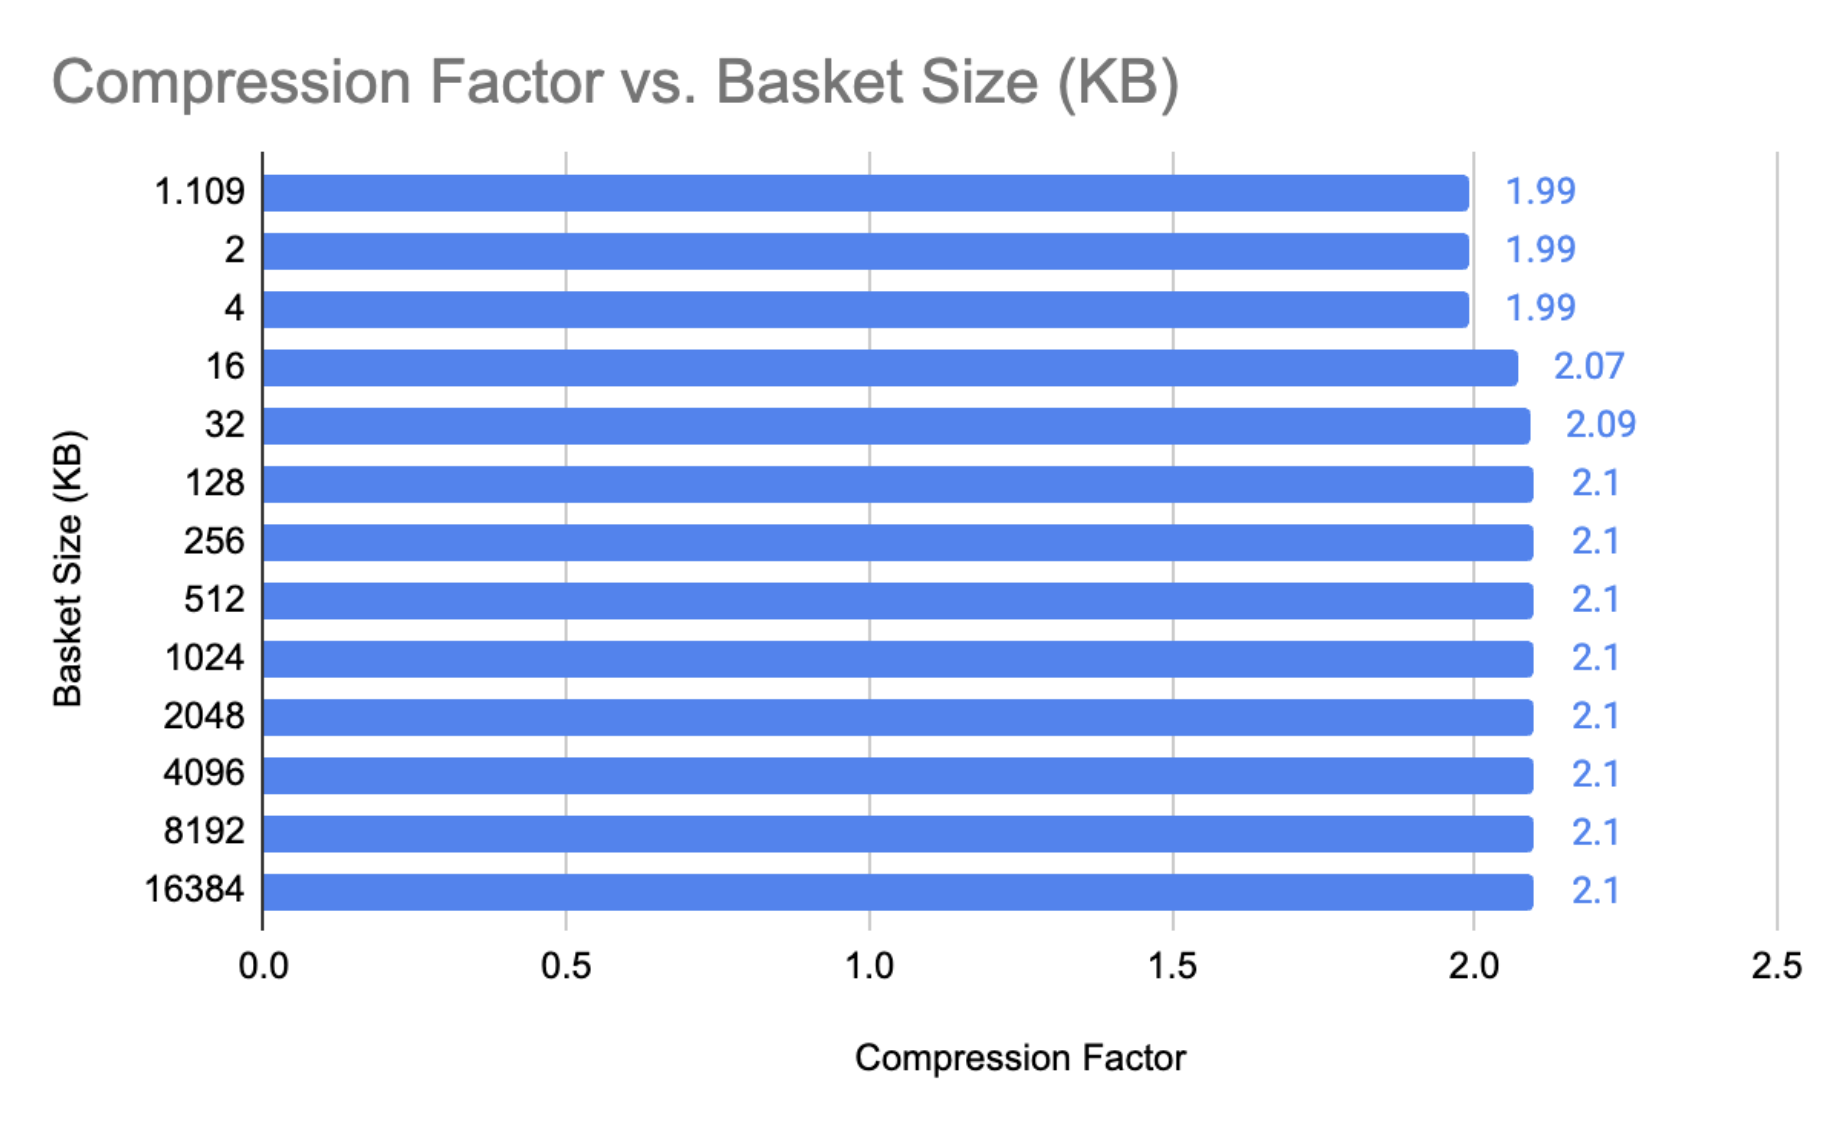
\includegraphics[width=.8\textwidth]{content/toymodel_content/Compression Factor vs. Branch Size (KB).png}
    \caption{Compression Factors vs Branch Size (1/2 Mixture $N=10^6$ events)}
    \label{fig:toymodel_CFvsBranchSize_1/2mixture}
\end{figure}

\begin{figure}[h]
    \centering
    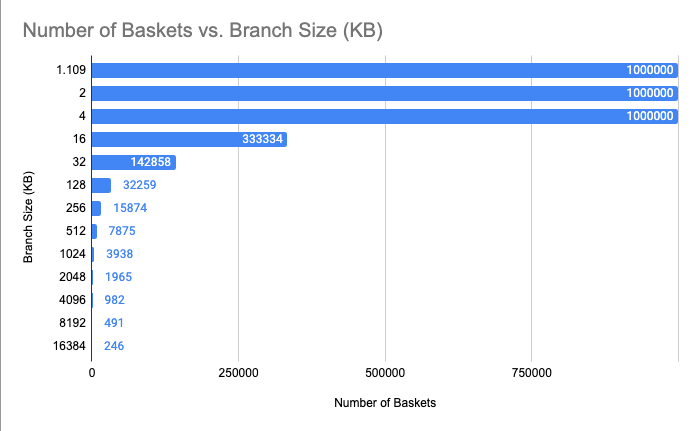
\includegraphics[width=.8\textwidth]{content/toymodel_content/Number of Baskets vs Branch Size.png}
    \caption{Number of Baskets vs Branch Size (1/2 Mixture $N=10^6$ events)}
    \label{fig:toymodel_NumBasketsvsBranchSize_1/2mixture}
\end{figure}

Figure \ref{fig:toymodel_CFvsBranchSize_1/2mixture} and Figure \ref{fig:toymodel_NumBasketsvsBranchSize_1/2mixture} is the first indication that the lower basket sizes are too small to effectively compress the data. 
For the baskets under 16 kB, it is required to have as many baskets as events to effectively store all the data--this will cause problems later on with memory usage so these basket sizes can be ignored.